\section{The Compute-Memory Trade-Off}
\sectionmark{Compute-Memory Trade-Off}

I demonstrate the compute-memory trade-off by showing for varying memory budget \(m\), what is the optimal computational cost the solver predicts.
`Simulated' in the \(y\) axis label refers to the fact that I am measuring what the solver `thinks', not that I am using the simulator instead of a real implementation.
I plot this for sequence lengths \(N\,=\, 20,\,40,\,100\), and vary \(m\) up to \(60\) for each.
I use a uniform network: the compute and memory costs of every forward and backward tensor is 1.

Starting from the right of the curve, we can see that compute cost degrades very slowly until \(m\) gets too low, then there is a visible `corner' and it degrades very fast.
However, this \(m\) is really quite low.
The following numbers are all read approximately from the graph.

We can see that for \(N\,=\,40\), the cost at the right of the curve, where \(m\,=\,60\), starts at just under 100.
\(m\) decreases all the way to just over 10 before we even see a 30\% overhead.
I postulate that, for a uniform network like this, the solver is keeping to at most one recomputation until the `corner'.
The costs are consistent with Chen's \(\Theta(\sqrt{N})\) analysis for one recomputation.

\begin{figure}[t]
    \centering
    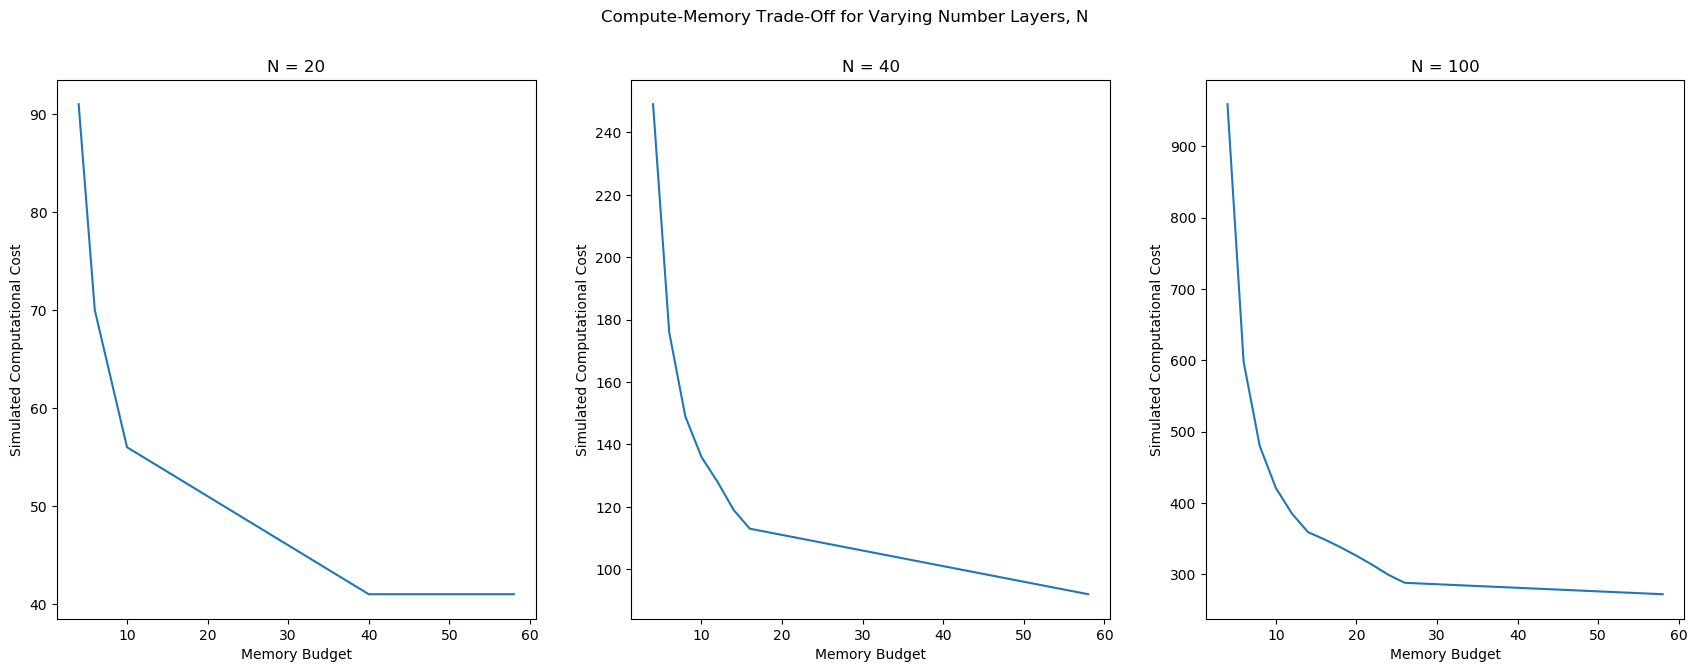
\includegraphics[width=0.9\linewidth]{compute_mem_tradeoff.png}
    \caption{The compute-memory trade-off for networks of different sequence length.}
    \label{fig:4-cm-tradeoff}
\end{figure}

For \(N\,=\,20\), the theoretical optimal memory consumption for uniform layers is \(2\sqrt{20}\,\approx\,9\).
We can see that it is at about \(m\,=\,9\) where the corner is encountered and the cost starts to quickly degrade.
This shows, primarly, how powerful even one recomputation is, as that is a signficant cost saving.
It also shows that, when given enough memory to not need to do more than one recomputation, the solver finds Chen's theoretical optimal policy.
However, Chen's solution simply picks a point on that curve, my solver is much more flexible.
It can make use of any extra memory to do less recomputation than the \(\Theta(\sqrt{N})\) approach, and, if memory gets too tight for that approach, it will find a policy that still satisfies the memory budget.
All of this is done automatically for the user.
In the extreme cases, we can see that for \(N\,=\,20\), at about \(m\,=\,40\) the curve flattens out, because there is now enough memory for \textit{no} recomputation to be required;
and on the other end of the graph, though at high cost, we see the solver is also able to satisfy \textit{very} small \(m\).
This will be due to it employing the quadratic-compute constant-memory `recompute everything' strategy.

In addition, the results across the three graphs show how well checkpointing scales to very deep networks.
For \(N\,=\,20\), reducing the memory budget from about 40 to 10, which is a 60\% reduction, gives a 38\% overhead.
For \(N\,=\,100\). reducing from about 60 to 24, which also is a 60\% reduction, gives hardly any visible effect.
Reducing all the way down to \(m\,=\,10\), a huge 83\% reduction, is required to observe a similar overhead of 40\%.
